
\chapter{Estimate Fusion on an Untrusted Cloud}\label{ch:cloud_fusion}

% 
% 8888888b.  8888888b.   .d88888b.  888888b.   
% 888   Y88b 888   Y88b d88P" "Y88b 888  "88b  
% 888    888 888    888 888     888 888  .88P  
% 888   d88P 888   d88P 888     888 8888888K.  
% 8888888P"  8888888P"  888     888 888  "Y88b 
% 888        888 T88b   888     888 888    888 
% 888        888  T88b  Y88b. .d88P 888   d88P 
% 888        888   T88b  "Y88888P"  8888888P"  
%                                              
%                                              
%                                              
% 

\section{Problem Formulation}\label{sec:cloud_fusion:problem}
%Our paper is motivated by a key step in multi-sensor fusion, the requirement of transmitting local sensor state estimates and covariance information over a network for the computation of their fused result. In particular, we consider centralized FCI fusion, where a party responsible for many networked sensors capable of computing their local state estimates, wishes to have their fused state estimate and covariance computed securely on an untrusted cloud. The same party may query the cloud fusion centre for the fused result at any time. To preserve the privacy of local sensor measurements and state estimates, we aim to provide a secure FCI algorithm such that the fusion centre does not learn individual sensor measurements, state estimates, or covariances. This will be achieved by encrypted homomorphic fusion, whereby the untrusted cloud learns only the FCI aggregation weights, which will be shown in section [sec:secfci].

%Our proposed filter aims to solve FCI fusion, namely () and (), using only encrypted values from each sensor $i$, and leaking only the weight values $\omega_1,\dots,\omega_n$.

%The problem of centralised fusion on a cloud server is a general


% TODO Add a sentence or two that follows well after the introduction section on the problem
% Then go straight into the definition

% TODO We fuse the information form. Note that that is also a goal (here only estimate and covariance are shown)

The concrete problem that we consider for cloud estimate fusion has been chosen for its broad applicability. We consider a discrete time-varying process defined by its state $\vec{x}_k \in \mathbb{R}^d$ at every timestep $k$. This process is estimated by sensors (or estimators) $i$, $1\leq i\leq n$, each producing a state estimate and estimate error covariance,
\begin{equation}\label{eq:cloud_fusion:sen_ests_and_covs}
    \hat{\vec{x}}_{k,i} \in \mathbb{R}^d \text{ and } \mat{P}_{k,i} \in \mathbb{R}^{d\times d}\,,
\end{equation}
respectively, at each timestep $k$. Our aim is for these estimates and their error covariances to be sent to a cloud server and fused, resulting in a fused estimate and estimate error covariance
\begin{equation}\label{eq:cloud_fusion:fus_ests_and_covs}
    \hat{\vec{x}}_{k,\mathsf{fus}} \in \mathbb{R}^d \text{ and } \mat{P}_{k,\mathsf{fus}} \in \mathbb{R}^{d\times d}\,,
\end{equation}
respectively, that are consistent with the estimates in \eqref{eq:cloud_fusion:sen_ests_and_covs}. That is, fused estimate error covariance is a conservative estimate of the optimal fused error covariance. In addition to the sensors and cloud fuser, a trusted third party can query the cloud for the fusion result \eqref{eq:cloud_fusion:fus_ests_and_covs} at any timestep $k$. The interactions between participants of the problem have been graphically summarised in figure \ref{fig:cloud_fusion:problem_layout}.
\begin{figure}[htbp]
    \centering
    \begin{tikzpicture}
        % Bounding box
        %\draw [gray] (1,-1.5) rectangle (8.5,7);
        % Estimators
        \node at (2.5,6.25) {Estimator $1$};
        \node at (7,6.25) {Estimator $n$};
        \fill [pyplotorange!70] (7,5.5) ellipse (0.5 and 0.5);
        \fill [pyplotorange!70] (2.5,5.5) ellipse (0.5 and 0.5);
        \fill [black] (5,5.5) circle (0.05);
        \fill [black] (4.5,5.5) circle (0.05);
        \fill [black] (4.75,5.5) circle (0.05);
        % Estimates
        \node [right] at (6.25,4.5) {$\hat{\vec{x}}_{k,m},\mat{P}_{k,n}$};
        \node [left] at (3.25,4.5) {$\hat{\vec{x}}_{k,1},\mat{P}_{k,1}$};
        % Fusion
        \node [right] at (5.25,0.5) {$\hat{\vec{x}}_{k,\mathsf{fus}},\mat{P}_{k,\mathsf{fus}}$};
        % Cloud
        \node at (4.75,3.65) {Cloud};
        \fill [pyplotorange!70] (4.75,3) ellipse (0.4 and 0.4);
        \fill [pyplotorange!70] (5.25,2.75) ellipse (0.4 and 0.25);
        \fill [pyplotorange!70] (4.25,2.75) ellipse (0.25 and 0.25);
        \fill [pyplotorange!70] (5.25,3) ellipse (0.25 and 0.25);
        \fill [pyplotorange!70] (4.25,2.5) rectangle (5.25,2.75);
        % Third party
        \node at (4.75,1.25) {Trusted Third party};
        \fill [pyplotblue!70] (5.5,-0.25) -- (4,-0.25) -- (4.75,1);
        % Estimator arrows
        \draw [-latex]  plot coordinates {(3,5)  (4.25,4)};
        \draw [-latex]  plot coordinates {(6.5,5)  (5.25,4)};
        % Third-party arrows
        \draw [latex-latex]  plot coordinates {(4.75,2.3)  (4.75,1.65)};
    \end{tikzpicture}
    \caption{Participants and communications in the considered cloud fusion problem.}
    \label{fig:cloud_fusion:problem_layout}
\end{figure}

In addition to the fusion of estimates, we specify the security goals of data fusion on an untrusted cloud. Both the cloud and sensors are considered \textit{honest-but-curious}, meaning they follow protocols correctly but may use any learned information for external malicious gain. The desire is for transmitted data accessible to the cloud and eavesdroppers to leak no additional information that is already known by the participants beyond formally specified leakage. Similarly, sensors should learn no additional information about transmitted data beyond their local estimates \eqref{eq:cloud_fusion:sen_ests_and_covs}. To achieve these goals, two methods are proposed in this chapter. The first allows complete homomorphic computation of the fusion results by the cloud but requires mutually trusted sensors and the leakage of relative error covariance sizes. The second method leaks no information in transmitted data and allows malicious collaborations, but requires additional computations by the trusted party when querying the cloud.

% 
% 8888888888 888     888  .d8888b. 8888888 .d88888b.  888b    888      888      
% 888        888     888 d88P  Y88b  888  d88P" "Y88b 8888b   888      888      
% 888        888     888 Y88b.       888  888     888 88888b  888      888      
% 8888888    888     888  "Y888b.    888  888     888 888Y88b 888      888      
% 888        888     888     "Y88b.  888  888     888 888 Y88b888      888      
% 888        888     888       "888  888  888     888 888  Y88888      888      
% 888        Y88b. .d88P Y88b  d88P  888  Y88b. .d88P 888   Y8888      888      
% 888         "Y88888P"   "Y8888P" 8888888 "Y88888P"  888    Y888      88888888 
%                                                                               
%                                                                               
%                                                                               
% 

\section{Confidential Cloud Fusion Leaking Fusion Weights}\label{sec:cloud_fusion:secfci}
In this section, we present the method for computing the fusion result \eqref{eq:cloud_fusion:fus_ests_and_covs} at the fusion cloud while leaking the order of sensor error covariances to the cloud and eavesdroppers. In addition to the layout in figure \ref{fig:cloud_fusion:problem_layout}, we assume that sensors are computationally capable of running both the Paillier and Lewi encryption schemes locally, from sections \ref{subsec:prelims:paillier} and \ref{subsec:prelims:lewi_ore}, respectively, and require a key distribution step before the beginning of the algorithm. Here, the trusted third party generates a Paillier scheme public key $\mathsf{pk}=N$ and secret key $\mathsf{sk}=(p,q)$ as well as a shared symmetric key $\mathsf{sk}_{\mathsf{o}}$ for the Lewi ORE scheme. The public key $\mathsf{pk}$ is made available to all participants in the fusion process, namely the cloud and sensors, while the shared ORE key $\mathsf{sk}_{\mathsf{o}}$ is made available only to the sensors and thus implies a trust between the sensors in this scenario. The sharing of these keys can be performed by any public-key encryption scheme such as RSA [rivestMethodObtainingDigital1978].
% TODO add discussion on the added assumption that sensors trust each other and that only the cloud is considered malicious

%As we assume the querying party is the owner of all individual sensors, the threat model to be considered is that of network eavesdroppers and a malicious fusion centre, with no possible collusion between sensors and the fusion centre.

% The benefit of leaking weights should be mentioned here. Allows for prioritising communication in bandwidth-limited scenarios.

% Desire IND-CPA except for leaked weights. Easier for the security section that follows.

% 
%  ######  ########  ######     ########  ######  #### 
% ##    ## ##       ##    ##    ##       ##    ##  ##  
% ##       ##       ##          ##       ##        ##  
%  ######  ######   ##          ######   ##        ##  
%       ## ##       ##          ##       ##        ##  
% ##    ## ##       ##    ##    ##       ##    ##  ##  
%  ######  ########  ######     ##        ######  #### 
% 

\subsection{Secure Fast Covariance Intersection}

% 
% ..#######...........######..########.##....##
% .##.....##.........##....##.##.......###...##
% ........##.........##.......##.......####..##
% ..#######..#######..######..######...##.##.##
% .##......................##.##.......##..####
% .##................##....##.##.......##...###
% .#########..........######..########.##....##
% 

\subsubsection{Two-sensor Case}\label{subsubsec:cloud_fusion:secfci_2sen}
The Secure Fast Covariance Intersection (SecFCI) fusion algorithm will first be introduced in the special case of two sensors, before an extension to the $n$-sensor case. Recalling FCI fusion \eqref{eq:prelims:ci_est}, \eqref{eq:prelims:ci_cov} and \eqref{eq:prelims:ci_weight_sum}, we can write the fusion of two estimates and their error covariances at timestep $k$ in the information form as
\begin{equation}
    \mat{P}_{k,\mathsf{fus}}^{-1}\hat{\vec{x}}_{k,\mathsf{fus}} = \omega_1\mat{P}_{k,1}^{-1}\hat{\vec{x}}_{k,1} + (1 - \omega_1)\mat{P}_{k,2}^{-1}\hat{\vec{x}}_{k,2}
\end{equation}
and
\begin{equation}
    \mat{P}_{k,\mathsf{fus}}^{-1} = \omega_1\mat{P}_{k,1}^{-1} + (1 - \omega_1)\mat{P}_{k,2}^{-1}\,,
\end{equation}
with $0\leq \omega_1\leq 1$, and note the suitability of addition and scalar multiplication to the Paillier scheme when the weight $\omega_1$ is known. To compute the fused information vector $\mat{P}_{k,\mathsf{fus}}^{-1}\hat{\vec{x}}_{k,\mathsf{fus}}$ and information matrix $\mat{P}_{k,\mathsf{fus}}^{-1}$ homomorphically, local estimate information must first be encoded as integers before encryption at the sensors. Using the Q number format, introduced in section \ref{subsec:prelims:encoding}, we let $M=N$, chose an appropriate precision $\phi$ and denote elementwise encoding with $d$ previous multiplications as $\mathsf{E}_d(\cdot)$. Encryption and fusion with Paillier homomorphic properties \eqref{eq:prelims:paillier_hom_add} and \eqref{eq:prelims:paillier_hom_mult} is then given by
\begin{equation}\label{eq:cloud_fusion:secfci_2sen_paillier_fuse_ests}
    \mathcal{E}_{\mathsf{pk}}\left(\mathsf{E}_1\left(\mat{P}_{k,\mathsf{fus}}^{-1}\hat{\vec{x}}_{k,\mathsf{fus}}\right)\right) \approx \mathcal{E}_{\mathsf{pk}}\left(\mathsf{E}_0\left(\mat{P}^{-1}_{k,1}\hat{\vec{x}}_{k,1}\right)\right)^{\mathsf{E}_0(\omega_1)}\mathcal{E}_{\mathsf{pk}}\left(\mathsf{E}_0\left(\mat{P}^{-1}_{k,2}\hat{\vec{x}}_{k,2}\right)\right)^{\mathsf{E}_0(1 - \omega_1)}\pmod{N}
\end{equation}
and
\begin{equation}\label{eq:cloud_fusion:secfci_2sen_paillier_fuse_covs}
    \mathcal{E}_{\mathsf{pk}}\left(\mathsf{E}_1\left(\mat{P}_{k,\mathsf{fus}}^{-1}\right)\right) \approx \mathcal{E}_{\mathsf{pk}}\left(\mathsf{E}_0\left(\mat{P}^{-1}_{k,1}\right)\right)^{\mathsf{E}_0(\omega_1)}\mathcal{E}_{\mathsf{pk}}\left(\mathsf{E}_0\left(\mat{P}^{-1}_{k,2}\right)\right)^{\mathsf{E}_0(1 -\omega_1)}\pmod{N}\,,
\end{equation}
with approximation errors caused by encoding and dependent on precision parameter $\phi$. The trusted querying party can now request encryptions \eqref{eq:cloud_fusion:secfci_2sen_paillier_fuse_ests} and \eqref{eq:cloud_fusion:secfci_2sen_paillier_fuse_covs} at any timestep $k$ and decrypt them to obtain the current fused information vector and information matrix and therefore the fused estimate and its error covariance.

All that remains for computing \eqref{eq:cloud_fusion:secfci_2sen_paillier_fuse_ests} and \eqref{eq:cloud_fusion:secfci_2sen_paillier_fuse_covs} in the two-sensor case is the calculation of parameter $\omega_1$ at the cloud. Since $\omega_1$ depends on the estimate errors of both sensors it cannot be computed locally and requires some leakage of the result to the cloud. We achieve this by using the Lewi ORE scheme and encrypting discretised sequences whose intersection can be used to compute the two-sensor FCI fusion weight constraint \eqref{eq:prelims:fci_added_constraints},
\begin{equation}\label{eq:cloud_fusion:secfci_2sen_intersect_cond}
    \omega_1\tr(\mat{P}_{k,1}) = (1-\omega_1)\tr(\mat{P}_{k,2})\,.
\end{equation}
To evaluate \eqref{eq:cloud_fusion:secfci_2sen_intersect_cond} with comparisons, we choose a stepsize $g\leq 1$, such that $1/g \in \mathbb{N}$, and both sensors discretise the weight $0\leq\omega_1\leq 1$ before computing the resulting sequences of either side of the equality in \eqref{eq:cloud_fusion:secfci_2sen_intersect_cond}. This results in the sequence
\begin{equation}\label{eq:cloud_fusion_secfci_2sen_seq_1}
    \left\langle0, g\tr(\mat{P}_{k,1}), 2g\tr(\mat{P}_{k,1}),\dots,\tr(\mat{P}_{k,1})\right\rangle
\end{equation}
at sensor $1$ and
\begin{equation}\label{eq:cloud_fusion_secfci_2sen_seq_2}
    \left\langle\tr(\mat{P}_{k,2}), (1-g)\tr(\mat{P}_{k,2}), (1-2g)\tr(\mat{P}_{k,2}),\dots,0\right\rangle
\end{equation}
at sensor $2$. Comparison of same-index values in the sequences \eqref{eq:cloud_fusion_secfci_2sen_seq_1} and \eqref{eq:cloud_fusion_secfci_2sen_seq_2} leads to the bounds $xg<\omega_1<(x+1)g$, for some index $x$, that can be used to approximate the true solution as $\hat{\omega}_1 = xg+ g/2 \approx \omega_1$, or in the case of an equality, $\hat{\omega}_1 = xg = \omega_1$. To obtain this approximation without additional leakage, elements in \eqref{eq:cloud_fusion_secfci_2sen_seq_1} and \eqref{eq:cloud_fusion_secfci_2sen_seq_2} are encrypted with the ORE key $\mathsf{sk}_{\mathsf{o}}$. As no homomorphic operations are performed with the scheme an arbitrary precision integer encoding can be used and is neglected from the notation below. The sequence produced by sensor $1$ is therefore given by
\begin{equation}\label{eq:cloud_fusion:secfci_2sen_enc_seq_1}
    \left\langle\mathcal{E}^{\mathsf{L}}_{\mathsf{sk}_{\mathsf{o}}}(0), \mathcal{E}^{\mathsf{L}}_{\mathsf{sk}_{\mathsf{o}}}(g\tr(\mat{P}_{k,1})), \mathcal{E}^{\mathsf{L}}_{\mathsf{sk}_{\mathsf{o}}}(2g\tr(\mat{P}_{k,1})),\dots,\mathcal{E}^{\mathsf{L}}_{\mathsf{sk}_{\mathsf{o}}}(\tr(\mat{P}_{k,1}))\right\rangle
\end{equation}
and that by sensor $2$ by
\begin{equation}\label{eq:cloud_fusion:secfci_2sen_enc_seq_2}
    \left\langle\mathcal{E}^{\mathsf{R}}_{\mathsf{sk}_{\mathsf{o}}}(\tr(\mat{P}_{k,2})), \mathcal{E}^{\mathsf{R}}_{\mathsf{sk}_{\mathsf{o}}}((1-g)\tr(\mat{P}_{k,2})), \mathcal{E}^{\mathsf{R}}_{\mathsf{sk}_{\mathsf{o}}}((1-2g)\tr(\mat{P}_{k,2})),\dots,\mathcal{E}^{\mathsf{R}}_{\mathsf{sk}_{\mathsf{o}}}(0)\right\rangle\,,
\end{equation}
where we note the difference between \textit{left} and \textit{right} encryptions for each sensor, allowing comparisons between sequences. Efficiently findable using a binary search, the approximate solution when comparing elements of the two sequences can be seen graphically in figure \ref{fig:cloud_fusion:secfci_2sen_intersect}, where the approximation is taken as halfway between consecutive comparisons that change sign.
\begin{figure}[htbp]
    \begin{center}
       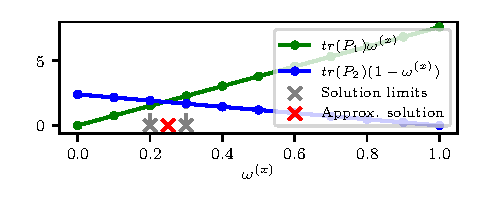
\includegraphics{figures/2_sensors.pdf}
    \end{center}
    \caption{Approximation of $\omega_1$ with stepsize $g=0.1$. Comparisons are only possible when $\omega_1$ is a multiple of $g$ (points on the graphs).}
    \label{fig:cloud_fusion:secfci_2sen_intersect}
    % TODO to figure. Y-axis should have 2 points, for trP1 and trP2. Omega^x should be omega_1. Make larger. Add a hat to the approximation of omega
 \end{figure}

In this way, computing fusion on the cloud homomorphically can be performed when having access to only local encryptions of information vectors and information matrices, \eqref{eq:cloud_fusion:secfci_2sen_paillier_fuse_covs} and \eqref{eq:cloud_fusion:secfci_2sen_paillier_fuse_ests}, in addition to the sequences of order-revealing encryptions \eqref{eq:cloud_fusion:secfci_2sen_enc_seq_1} and \eqref{eq:cloud_fusion:secfci_2sen_enc_seq_2} that leak an approximation $\hat{\omega}_1 \approx \omega_1$.

% 
% .##....##..........######..########.##....##
% .###...##.........##....##.##.......###...##
% .####..##.........##.......##.......####..##
% .##.##.##.#######..######..######...##.##.##
% .##..####...............##.##.......##..####
% .##...###.........##....##.##.......##...###
% .##....##..........######..########.##....##
% 

\subsubsection{Multi-sensor Case}\label{subsubsec:cloud_fusion:secfci_nsen}
To compute the fusion of $n$ sensor estimates in the information form we want the solutions to
\begin{equation}
    \mat{P}_{k,\mathsf{fus}}^{-1}\hat{\vec{x}}_{k,\mathsf{fus}} = \sum_{i=1}^n\omega_i\mat{P}_{k,i}^{-1}\hat{\vec{x}}_{k,i}
\end{equation}
and
\begin{equation}
    \mat{P}_{k,\mathsf{fus}}^{-1} = \sum_{i=1}^n\omega_i\mat{P}_{k,i}^{-1}\,.
\end{equation}
When the fusion weights $\omega_i$, $1\leq i\leq n$, $\sum_{i=1}^n\omega_i=1$, are known, we can again use the appropriate integer encoding and Paillier homomorphic properties to compute the fusion homomorphically as
\begin{equation}\label{eq:cloud_fusion:secfci_nsen_paillier_fuse_ests}
    \mathcal{E}_{\mathsf{pk}}\left(\mathsf{E}_1\left(\mat{P}_{k,\mathsf{fus}}^{-1}\hat{\vec{x}}_{k,\mathsf{fus}}\right)\right) \approx \prod_{i=1}^n\mathcal{E}_{\mathsf{pk}}\left(\mathsf{E}_0\left(\mat{P}^{-1}_{k,i}\hat{\vec{x}}_{k,i}\right)\right)^{\mathsf{E}_0(\omega_i)}\pmod{N}
\end{equation}
and
\begin{equation}\label{eq:cloud_fusion:secfci_nsen_paillier_fuse_covs}
    \mathcal{E}_{\mathsf{pk}}\left(\mathsf{E}_1\left(\mat{P}_{k,\mathsf{fus}}^{-1}\right)\right) \approx \prod_{i=1}^n\mathcal{E}_{\mathsf{pk}}\left(\mathsf{E}_0\left(\mat{P}^{-1}_{k,i}\right)\right)^{\mathsf{E}_0(\omega_i)}\,.
\end{equation}
What remains is to compute the weights $\omega_i$ at the cloud such that the $n$-sensor FCI conditions \eqref{eq:prelims:fci_added_constraints} are met. Similar to the two-sensor case, we can use sequences of order-revealing encryptions to leak an approximation to this result. 

Each condition \eqref{eq:prelims:fci_added_constraints} is considered as a partial problem, that is,
\begin{equation}\label{eq:cloud_fusion:secfci_nsen_partial_sol_subspace}
    \omega_i\tr(\mat{P}_{k,i}) = \omega_{i+1}\tr(\mat{P}_{k,i+1})\,,
\end{equation}
with $1\leq i< n$ and $\sum_{i=1}^n\omega_i=1$, and their solution spaces, linear subspaces $\mathcal{S}_i$ over possible values of $\vec{\omega}=\begin{bsmallmatrix}\omega_1 & \cdots & \omega_n\end{bsmallmatrix}^\top$, desired. The intersection of these subspaces naturally results in the final solution to $\vec{\omega}$ in \eqref{eq:prelims:fci_matrix_equation}. Each solution space $\mathcal{S}_i$ can be defined by $n-1$ contained and linearly independent solutions $\vec{\omega}_i^{(s)}$, $1\leq s\leq n-1$. $n-2$ of these solutions can be trivially obtained as the points where a single $\omega_j=1$, $j\neq i\neq i+1$ while the final point, $\vec{\omega}_i^{(n-1)}$, can be obtained as the solution to
\begin{equation}\label{eq:cloud_fusion:secfci_nsen_partial_sol_point}
    \omega_i\tr(\mat{P}_{k,i}) = (1-\omega_i)\tr(\mat{P}_{k,i+1})\,,
\end{equation}
$\omega_j=0$, $j\neq i\neq i+1$, noting equivalence to \eqref{eq:cloud_fusion:secfci_nsen_partial_sol_subspace} and $\omega_{i+1}=1-\omega_i$. The solutions $\vec{\omega}_i^{(s)}$ and the $n-2$ dimensional subspace they define can be rewritten in parametric form as
\begin{equation}\label{eq:cloud_fusion:secfci_nsen_partial_subspace}
    \mathcal{S}_i(\vec{\gamma}_i)=\vec{\omega}_i^{(1)} + 
    \begin{bmatrix}
        \bar{\vec{\omega}}_i^{(2)} & \cdots & \bar{\vec{\omega}}_i^{(n-1)}
    \end{bmatrix}
    \vec{\gamma}_i\,,
\end{equation}
where $\bar{\vec{\omega}}_i^{(x)}=\vec{\omega}_i^{(x)}-\vec{\omega}_i^{(1)}$ denotes the direction vectors. The intersection of these $n-1$ subspaces gives the solution to $\vec{\omega}$ in \eqref{eq:prelims:fci_matrix_equation}. This solution, as well as the parameters $\vec{\gamma}_i$, can be obtained as a solution to the linear system
\begin{equation}\label{eq:cloud_fusion:secfci_nsen_omega_solution}
    \begin{bmatrix}
        -\mat{I} & \bar{\vec{\omega}}_1^{(2)} & \cdots & \bar{\vec{\omega}}_1^{(n-1)} & 0 & \cdots & 0\\
        \vdots & 0 &  & \ddots &  & \ddots & \vdots\\
        \vdots & \vdots & \ddots &  & \ddots &  & 0\\
        -\mat{I} & 0 & \cdots & 0 & \bar{\vec{\omega}}_{n-1}^{(2)} & \cdots & \bar{\vec{\omega}}_{n-1}^{(n-1)}
    \end{bmatrix}
    \begin{bmatrix}
        \vec{\omega}\\
        \vec{\gamma}_1\\
        \vdots\\
        \vec{\gamma}_{n-1}\\
    \end{bmatrix}=
    \begin{bmatrix}
        -\vec{\omega}_1^{(1)}\\
        \vdots\\
        -\vec{\omega}_{n-1}^{(1)}\\
    \end{bmatrix}\,.
\end{equation}

Therefore, to compute \eqref{eq:cloud_fusion:secfci_nsen_omega_solution} at the cloud without leaking more than comparisons, we approximate the solutions to \eqref{eq:cloud_fusion:secfci_nsen_partial_sol_point} with ORE sequences similar to the two-sensor case. Each sensor $i$ uses $\mathsf{sk}_{\mathsf{o}}$ to encrypt the discretisation 
\begin{equation}\label{eq:cloud_fusion:secfci_nsen_enc_seqs}
    \begin{split}
        \left\langle\mathcal{E}^{\mathsf{L}}_{\mathsf{sk}_{\mathsf{o}}}(0), \mathcal{E}^{\mathsf{L}}_{\mathsf{sk}_{\mathsf{o}}}(g\tr(\mat{P}_{k,i})), \mathcal{E}^{\mathsf{L}}_{\mathsf{sk}_{\mathsf{o}}}(2g\tr(\mat{P}_{k,i})),\dots,\mathcal{E}^{\mathsf{L}}_{\mathsf{sk}_{\mathsf{o}}}(\tr(\mat{P}_{k,i}))\right\rangle\,,\ & \text{if } i \text{ is odd, or}\\
        \left\langle\mathcal{E}^{\mathsf{R}}_{\mathsf{sk}_{\mathsf{o}}}(0), \mathcal{E}^{\mathsf{R}}_{\mathsf{sk}_{\mathsf{o}}}(g\tr(\mat{P}_{k,i})), \mathcal{E}^{\mathsf{R}}_{\mathsf{sk}_{\mathsf{o}}}(2g\tr(\mat{P}_{k,i})),\dots,\mathcal{E}^{\mathsf{R}}_{\mathsf{sk}_{\mathsf{o}}}(\tr(\mat{P}_{k,i}))\right\rangle\,,\ & \text{if } i \text{ is even,}
    \end{split}
\end{equation}
allowing for comparison between sequences from consecutive sensors $i$ and $i+1$. To approximate the solution to each \eqref{eq:cloud_fusion:secfci_nsen_partial_sol_point}, the sequence from sensor $i+1$ is reversed,
\begin{equation}\label{eq:cloud_fusion:secfci_nsen_enc_seqs_reversed}
    \begin{split}
        \left\langle\mathcal{E}^{\mathsf{L}}_{\mathsf{sk}_{\mathsf{o}}}(\tr(\mat{P}_{k,i})),\mathcal{E}^{\mathsf{L}}_{\mathsf{sk}_{\mathsf{o}}}((1-g)\tr(\mat{P}_{k,i})), \mathcal{E}^{\mathsf{L}}_{\mathsf{sk}_{\mathsf{o}}}((1-2g)\tr(\mat{P}_{k,i})),\dots,\mathcal{E}^{\mathsf{L}}_{\mathsf{sk}_{\mathsf{o}}}(0)\right\rangle\,,\ & \text{if } i \text{ is odd, or}\\
        \left\langle\mathcal{E}^{\mathsf{R}}_{\mathsf{sk}_{\mathsf{o}}}(\tr(\mat{P}_{k,i})), \mathcal{E}^{\mathsf{R}}_{\mathsf{sk}_{\mathsf{o}}}((1-g)\tr(\mat{P}_{k,i})), \mathcal{E}^{\mathsf{R}}_{\mathsf{sk}_{\mathsf{o}}}((1-2g)\tr(\mat{P}_{k,i})),\dots,\mathcal{E}^{\mathsf{R}}_{\mathsf{sk}_{\mathsf{o}}}(0)\right\rangle\,,\ & \text{if } i \text{ is even,}
    \end{split}
\end{equation}
resulting in sequences of the same form as \eqref{eq:cloud_fusion:secfci_2sen_enc_seq_1} and \eqref{eq:cloud_fusion:secfci_2sen_enc_seq_2}. The value $\hat{\omega}_i = xg + g/2 \approx \omega_i$, or in the case of an equality $\hat{\omega}_i = xg = \omega_i$, for some index $x$, is used to approximate the solution $\hat{\vec{\omega}}_i^{(n-1)} \approx \vec{\omega}_i^{(n-1)}$. A visualisation of solving \eqref{eq:cloud_fusion:secfci_nsen_omega_solution} with approximations to \eqref{eq:cloud_fusion:secfci_nsen_partial_sol_point} in the three-sensor has case is graphically displayed in figure \ref{fig:cloud_fusion:secfci_nsen_partial_sols_and_intersect}.
\begin{figure}[htbp]
    \begin{subfigure}[htbp]{\textwidth}
        \begin{center}
            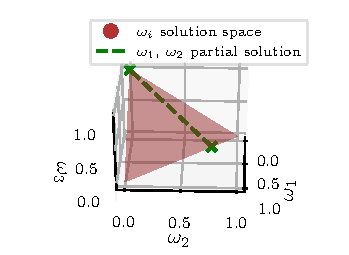
\includegraphics{figures/partial_sol1.pdf}
        \end{center}
        \caption{Approximated solution space \eqref{eq:cloud_fusion:secfci_nsen_partial_subspace} when $i=1$.}
        \label{fig:3_sensor_partial_sol}
    \end{subfigure}
    \hfill
    \begin{subfigure}[htbp]{\textwidth}
        \begin{center}
            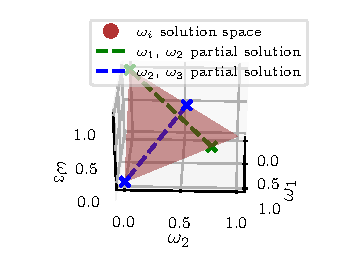
\includegraphics{figures/partial_sols.pdf}
        \end{center}
        \caption{Approximated solution space \eqref{eq:cloud_fusion:secfci_nsen_partial_subspace} when $i=2$.}
        \label{fig:3_sensor_partial_sols}
    \end{subfigure}
    \hfill
    \begin{subfigure}[htbp]{\textwidth}
        \begin{center}
            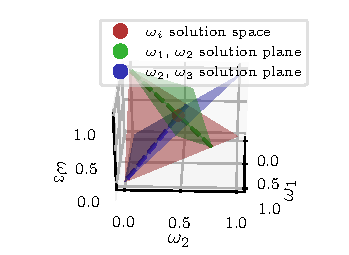
\includegraphics{figures/partial_sol_planes.pdf}
        \end{center}
        \caption{Intersection of partial solutions spaces gives fusion weights $\vec{\omega}$ in \eqref{eq:prelims:fci_matrix_equation}.}
        \label{fig:3sen_planes}
    \end{subfigure}
    \caption{Solving fusion weights $\vec{\omega}$ with approximations to \eqref{eq:cloud_fusion:secfci_nsen_partial_sol_point}.}
    \label{fig:cloud_fusion:secfci_nsen_partial_sols_and_intersect}
    % TODO Label which points are approximated. Turn axis labels the right way around. Label solution space correctly; it is the plane of the sum equalling one.
\end{figure}

The resulting estimate $\hat{\vec{\omega}} \approx \vec{\omega}$ can then be used with \eqref{eq:cloud_fusion:secfci_nsen_paillier_fuse_ests} and \eqref{eq:cloud_fusion:secfci_nsen_paillier_fuse_covs} to compute the fusion of $n$ estimates in information form at the cloud.

% 
%  ######   #######  ##     ## ########  
% ##    ## ##     ## ###   ### ##     ## 
% ##       ##     ## #### #### ##     ## 
% ##       ##     ## ## ### ## ########  
% ##       ##     ## ##     ## ##        
% ##    ## ##     ## ##     ## ##        
%  ######   #######  ##     ## ##        
% 

\subsection{Computational Complexity}\label{subsec:cloud_fusion:secfci_comp_complexity}
The method introduced allows the computation of FCI at a cloud by homomorphically fusing $n$ sensor states estimated with leaked fusion weights using the Paillier and Lewi encryption schemes. Naturally, relying on encryption and homomorphic operations increases the complexity of computing this fusion at the sensor, cloud and querying party. Here, we look at the computational complexity of the method in terms of the required operations at each party for each timestep $k$. We assume that both the Lewi and Paillier schemes use the same key size, typically measured in bits, $\log{N}$, where $N$ is the Paillier modulus in section \ref{subsec:prelims:paillier}. In addition, we note the distinction between floating-point or small integer operations, treated as having runtime $O(1)$, and large integer operations with runtime dependent on bit length. While hardware architecture exists for faster encryption operations [gueronIntelAdvancedEncryption2010], we consider software implementations and treat large integer operations in terms of bit operations explicitly.

Individual encryption operation complexities with the assumptions made above have been summarised in table \ref{tab:cloud_fusion:secfci_op_complexity}. 
\begin{table}[htbp]
    \centering
    \caption{Computation complexity of involved encryption operations.}
    \label{tab:cloud_fusion:secfci_op_complexity}
    \begin{tabular}{|c|c|}
        \hline
        \textbf{Operation} & \textbf{Complexity} \\ 
        \hline
        Paillier Encryption & $O(\log^3{N})$ \\ 
        Paillier Decryption & $O(\log^3{N})$ \\ 
        Paillier Addition & $O(\log^2{N})$ \\ 
        Paillier Scalar Multiplication & $O(\log^3{N})$ \\ 
        Lewi \textit{Left} Encryption & $O(\log^2{N})$ \\ 
        Lewi \textit{Right} Encryption & $O(\log^2{N})$ \\ 
        Lewi Comparison & $O(\log^2{N})$ \\ 
        \hline
    \end{tabular}
\end{table}
Applying operation complexities to the fusion algorithm we get the computational complexity for the sensors, cloud and querying party. These can be seen in table \ref{tab:cloud_fusion:secfci_complexity}, where unencrypted FCI algorithm complexities are also shown for reference. 
\begin{table}[htbp]
   \centering
   \caption{Computation complexity at each timestep $k$ for each party.}
   \label{tab:cloud_fusion:secfci_complexity}
   \begin{tabular}{|c|c|c|}
      \hline
       & \textbf{FCI} & \textbf{Confidential Fusion Leaking Weights} \\ 
      \hline
      Sensor & $O(1)$ & $O\left(d^2\log^3{N} + \frac{1}{g}\log^2{N}\right)$ \\ 
      Cloud & $O(nd^2+n^3)$ & $O\left(nd^2\log^3{N} + n\log{\frac{1}{g}} + n^3\right)$ \\ 
      Querying Party & $O(1)$ & $O\left(d^2\log^3{N}\right)$ \\ 
      \hline
   \end{tabular}
\end{table}
These complexities show the additional computational cost required for providing the security benefits of the presented scheme and must naturally be reflected in chosen hardware when developing a system where the benefits are desired.

% 
%  ######  ########  ######  
% ##    ## ##       ##    ## 
% ##       ##       ##       
%  ######  ######   ##       
%       ## ##       ##       
% ##    ## ##       ##    ## 
%  ######  ########  ######  
% 

\subsection{Security Analysis}\label{subsec:cloud_fusion:secfci_security}
To discuss the security of the presented scheme we look at the assumptions on collusions between participants and the cryptographic guarantees of the used encryption schemes. As we require that all sensors share the ORE secret key $\mathsf{sk}_{\mathsf{o}}$, we assume trust between the sensors in the case of cloud fusion when leaking fusion weights. The cloud and eavesdroppers are not trusted by the sensors and can only gain access to the Paillier encryptions of estimates, \eqref{eq:cloud_fusion:secfci_nsen_paillier_fuse_ests} and \eqref{eq:cloud_fusion:secfci_nsen_paillier_fuse_covs}, and the Lewi ORE encrypted sequences \eqref{eq:cloud_fusion:secfci_nsen_enc_seqs}.

Since Paillier encryptions \eqref{eq:cloud_fusion:secfci_nsen_paillier_fuse_ests} and \eqref{eq:cloud_fusion:secfci_nsen_paillier_fuse_covs} meet the IND-CPA notion, estimates themselves are indistinguishable to the cloud and eavesdroppers as desired by our security goals. The leakage from the Lewi encrypted sequences is captured by the simulation-based security met by the scheme. This is shown in section \ref{subsubsec:cloud_fusion:secfci_nsen} to be a function of leaking approximations to the weights $\omega_i$ and therefore the relative uncertainties of sensors, in addition to some leakage beyond ciphertext ordering, due to the relaxation of the IND-OCPA notion, which can be difficult to quantify. Lastly, we also acknowledge the implicit leakage of state dimension $d$ associated with elementwise encryption. Although methods for homomorphic encryption of vectors exist [alexandruPrivateWeightedSum2020], we leave this as future work on this topic and note that the dimension $d$ may leak information about the data fusion use case but the state estimates themselves remain hidden.

Due to leaking relative sensor uncertainties, this method leaks confidential information that may lead to inferences about sensor hardware. However, this leakage also has the upside of benefitting fusion performance by allowing the cloud to prioritise the fusion of some sensor data over others. For example, in bandwidth-limited networks, communication with sensors of higher uncertainty may be dropped in favour of those that lead to better fusion results.

% 
%  ######  #### ##     ## 
% ##    ##  ##  ###   ### 
% ##        ##  #### #### 
%  ######   ##  ## ### ## 
%       ##  ##  ##     ## 
% ##    ##  ##  ##     ## 
%  ######  #### ##     ## 
% 

\subsection{Simulation}\label{subsec:cloud_fusion:secfci_simulation}
Lastly, along with the discussions above, we have implemented a simulation of the method to demonstrate its fusion accuracy when compared to the FCI algorithm on a trusted cloud. A constant-speed linear system, 
\begin{equation}\label{eq:cloud_fusion:secfci_system_model}
    \vec{x}_{k+1} = 
    \begin{bmatrix}
        1 & 0.5 & 0 & 0\\
        0 & 1 & 0 & 0\\
        0 & 0 & 1 & 0.5\\
        0 & 0 & 0 & 1
    \end{bmatrix}\vec{x}_k + \vec{w}_k\,,\qquad \vec{w}_k\sim\mathcal{N}\left(\vec{0},
    \begin{bmatrix}
        0.4 & 1.3 & 0 & 0\\
        1.3 & 5.0 & 0 & 0\\
        0 & 0 & 0.4 & 1.3\\
        0 & 0 & 1.3 & 5.0
    \end{bmatrix}
    \right)\,,
\end{equation}
is simulated and measured by three independent position sensors $1\leq i\leq 3$, producing measurements 
\begin{equation}\label{eq:cloud_fusion:secfci_measurement_model}
    \vec{z}_{k,i} = 
    \begin{bmatrix}
        1 & 0 & 0 & 0\\
        0 & 0 & 1 & 0
     \end{bmatrix}\vec{x}_k + \vec{v}_{k,i}\,,\qquad \vec{v}_{k,i}\sim\mathcal{N}\left(\vec{0},\mat{R}_i\right)\,,
\end{equation}
with
\begin{equation}
    \mat{R}_1=
    \begin{bmatrix}
        5 & 2\\
        2 & 5
    \end{bmatrix}\,,\ 
    \mat{R}_2=
    \begin{bmatrix}
        7 & 2\\
        2 & 4
    \end{bmatrix}\text{ and }
    \mat{R}_3=
    \begin{bmatrix}
        5 & 4\\
        4 & 8
    \end{bmatrix}\,.
\end{equation}
Each sensor runs a local linear Kalman Filter (KF) from section \ref{subsec:prelims:kf} before its information is sent to a server for fusion and in encrypted cases decrypted by a querying party. Figure \ref{fig:cloud_fusion:secfci_sim_error} shows the average estimation error of $1000$ simulations when using our algorithm with varying stepsizes $g$ alongside the standard FCI algorithm. 
\begin{figure}[htbp]
    \centering
    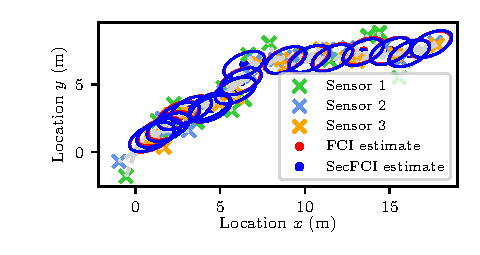
\includegraphics{figures/fci_secfci_cmp.pdf}
    \caption{Estimation error with varying stepsize $g$.}
    \label{fig:cloud_fusion:secfci_sim_error}
    % TODO figure to display MSE of 1000 simulations for FCI and our method with g=0.1, 0.2, 0.33, 0.5
    % latex y-axis label for MSE
 \end{figure}
 In all cases, resulting plaintext information vectors and matrices are converted to estimates and estimate error covariances before comparison with the true simulated state. From the figure, it can be seen that the estimation error of our method is similar to the normal FCI method when stepsize $g$ is small, $g\leq 2$, but grows as expected when $g$, and thus the possible error in weights $\omega_i$, is increased.

Since the system described by \eqref{eq:cloud_fusion:secfci_system_model}, \eqref{eq:cloud_fusion:secfci_measurement_model} and estimated by the KF reaches an estimation steady-state, fusion weights $\omega_i$ do as well. Figure \ref{fig:cloud_fusion:secfci_omega_error} shows the steady state error of estimated weights when compared to the true FCI weights. 
\begin{figure}[htbp]
    \centering
    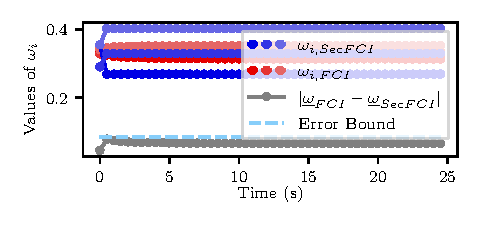
\includegraphics{figures/omegas_cmp.pdf}
    \caption{Error of estimated weights $\hat{\vec{\omega}}$ with varying stepsize $g$.}
    \label{fig:cloud_fusion:secfci_omega_error}
    % TODO plot steady-state error of weights g=0.1,0,2,0.33,0.5
    % Y-axis is weight error (not simulation error) and X-axis is g
\end{figure}
Here, the maximum errors in fusion weights naturally depend on the stepsize $g$ and support the results seen in figure \ref{fig:cloud_fusion:secfci_sim_error}. Further, an upper bound on this error can be derived by considering the maximum error of each approximation \eqref{eq:cloud_fusion:secfci_nsen_partial_sol_point} and is given by
\begin{equation}
    \left|\hat{\vec{\omega}} - \vec{\omega}\right| \leq \frac{g}{2}\sqrt{n}\,.
\end{equation}

% 
% 8888888888 888     888  .d8888b. 8888888 .d88888b.  888b    888      888b    888 888      
% 888        888     888 d88P  Y88b  888  d88P" "Y88b 8888b   888      8888b   888 888      
% 888        888     888 Y88b.       888  888     888 88888b  888      88888b  888 888      
% 8888888    888     888  "Y888b.    888  888     888 888Y88b 888      888Y88b 888 888      
% 888        888     888     "Y88b.  888  888     888 888 Y88b888      888 Y88b888 888      
% 888        888     888       "888  888  888     888 888  Y88888      888  Y88888 888      
% 888        Y88b. .d88P Y88b  d88P  888  Y88b. .d88P 888   Y8888      888   Y8888 888      
% 888         "Y88888P"   "Y8888P" 8888888 "Y88888P"  888    Y888      888    Y888 88888888 
%                                                                                           
%                                                                                           
%                                                                                           
% 

\section{Confidential Cloud Fusion Without Leaking Fusion Weights}\label{sec:cloud_fusion:secfci2}
In section \ref{sec:cloud_fusion:secfci} we introduced a solution to the cloud fusion problem that solves confidential estimate fusion on an untrusted cloud under some additional assumptions on the system. Namely, we assumed that the sensors were mutually trusted and allowed the leakage of fusion weights $\omega_i$, $1\leq i\leq n$, at the cloud, in turn allowing the cloud to prioritise estimates at the cost of leaking confidential information. Here, we propose an alternative method that relaxes these assumptions, providing estimate fusion without assuming trust between the sensors or allowing leakage of fusion weights. 

The idea of the method is to postpone the evaluation of operations that cannot be performed homomorphically until partial results are decrypted by the querying party. The remaining operations can then be evaluated on unencrypted inputs to produce the final results. First, we note that FCI fusion \eqref{eq:prelims:ci_est}, \eqref{eq:prelims:ci_cov} and \eqref{eq:prelims:fci_solution} can be rearranged and weights substituted to obtain
\begin{equation}\label{eq:cloud_fusion:secfci2_est_rearrange}
    \hat{\vec{x}}_{k,\mathsf{fus}} = \mat{P}_{k,\mathsf{fus}}\left(\sum_{i=1}^n \frac{1}{\tr(\mat{P}_{k,i})}\right)^{-1}\sum_{i=1}^n\frac{1}{\tr(\mat{P}_{k,i})}\mat{P}_{k,i}^{-1}\hat{\vec{x}}_{k,i}
\end{equation}
and
\begin{equation}\label{eq:cloud_fusion:secfci2_cov_rearrange}
    \mat{P}_{k,\mathsf{fus}} = \left(\left(\sum_{i=1}^n \frac{1}{\tr(\mat{P}_{k,i})}\right)^{-1}\sum_{i=1}^n \frac{1}{\tr(\mat{P}_{k,i})}\mat{P}_{k,i}^{-1}\right)^{-1}\,.
\end{equation}

In this form, innermost summations  
\begin{equation}
    \sum_{i=1}^n \frac{1}{\tr(\mat{P}_{k,i})}\,,\ \sum_{i=1}^n \frac{1}{\tr(\mat{P}_{k,i})}\mat{P}_{k,i}^{-1}\text{ and }\sum_{i=1}^n\frac{1}{\tr(\mat{P}_{k,i})}\mat{P}_{k,i}^{-1}\hat{\vec{x}}_{k,i}
\end{equation}
combine information from individual sensors $i$ and are computable homomorphically given suitable encryptions. Encryptions of these sums can then be decrypted by the querying party, before remaining inversions and multiplications in \eqref{eq:cloud_fusion:secfci2_est_rearrange} and \eqref{eq:cloud_fusion:secfci2_cov_rearrange} can be computed to obtain the final results. To depict this process, pseudocode for the encryption at the sensors, fusion at the cloud and decryption at the querying party are shown in algorithms \ref{alg:cloud_fusion:secfci2_sensor_steps}, \ref{alg:cloud_fusion:secfci2_cloud_steps} and \ref{alg:cloud_fusion:secfci2_query_steps}, respectively. As in the previous section, encoding from section \ref{subsec:prelims:encoding} is used with $M=N$, where $N$ is the Paillier scheme public key, and an appropriate precision $\phi$ is chosen.
\begin{algorithm}[htbp]
\caption{Encryption at Sensors}\label{alg:cloud_fusion:secfci2_sensor_steps}
\begin{algorithmic}[1]
    \setstretch{1.35}
    \Procedure{Estimate}{$i$, $k$, $\mathsf{pk}$}
    \State Estimate $\mat{P}_{k,i}^{-1}\hat{\vec{x}}_{k,i}$ locally
    \State Estimate $\mat{P}_{k,i}^{-1}$ locally
    \LineComment{Encode and encrypt scaling, covariance and estimate components}
    \State $s_{k,i} \gets \mathcal{E}_{\mathsf{pk}}\left(\mathsf{E}_{0}\left(\frac{1}{\tr(\mat{P}_{k,i})}\right)\right)$
    \State $\mat{C}_{k,i} \gets \mathcal{E}_{\mathsf{pk}}\left(\mathsf{E}_{0}\left(\frac{1}{\tr(\mat{P}_{k,i})}\mat{P}_{k,i}^{-1}\right)\right)$
    \State $\vec{e}_{k,i} \gets \mathcal{E}_{\mathsf{pk}}\left(\mathsf{E}_{0}\left(\frac{1}{\tr(\mat{P}_{k,i})}\mat{P}_{k,i}^{-1}\hat{\vec{x}}_{k,i}\right)\right)$
    \State Send $s_{k,i}$, $\mat{C}_{k,i}$ and $\vec{e}_{k,i}$ to fusing cloud
    \EndProcedure
\end{algorithmic}
\end{algorithm}
\begin{algorithm}[htbp]
\caption{Partial Fusion at the Cloud}\label{alg:cloud_fusion:secfci2_cloud_steps}
\begin{algorithmic}[1]
    \setstretch{1.35}
    \Procedure{PartialFuse}{$k$, $\mathsf{pk}$}
    \State Receive $s_{k,i}$, $\mat{C}_{k,i}$ and $\vec{e}_{k,i}$ for all $1\leq i \leq m$
    \LineComment{Public key is encryption modulus}
    \State $N \gets \mathsf{pk}$
    \LineComment{Perform homomorphic summations}
    \State $s_k \gets \prod_{i=1}^{m} s_{k,i} \pmod{N^2}$
    \State $\mat{C}_k \gets \otimes_{i=1}^{m} \mat{C}_{k,i} \pmod{N^2}$
    \State $\vec{e}_k \gets \otimes_{i=1}^{m} \vec{e}_{k,i} \pmod{N^2}$
    \State Store $s_k$, $\mat{C}_k$ and $\vec{e}_k$ in case of query
    \EndProcedure
\end{algorithmic}
\end{algorithm}
\begin{algorithm}[htbp]
\caption{Completing Fusion at the Querying Party}\label{alg:cloud_fusion:secfci2_query_steps}
\begin{algorithmic}[1]
    \setstretch{1.35}
    \Procedure{QueryFuse}{$k$, $\mathsf{pk}$, $\mathsf{sk}$}
    \State Query and receive $s_k$, $\mat{C}_k$ and $\vec{e}_k$ from fusing cloud
    \State $N \gets \mathsf{pk}$
    \LineComment Decrypt and decode
    \State $\bar{s}_k \gets \mathsf{E}^{-1}_{0}\left(\mathcal{D}_{\mathsf{sk}}\left(s_k\right)\right)$
    \State $\bar{\mat{C}}_k \gets \mathsf{E}^{-1}_{0}\left(\mathcal{D}_{\mathsf{sk}}\left(\mat{C}_k\right)\right)$
    \State $\bar{\vec{e}}_k \gets \mathsf{E}^{-1}_{0}\left(\mathcal{D}_{\mathsf{sk}}\left(\vec{e}_k\right)\right)$
    \LineComment Compute remaining fusion operations
    \State $\mat{P}_{k,\mathsf{fus}}^{-1} \gets \bar{s}_k^{-1} \cdot \bar{\mat{C}}_k$
    \State $\mat{P}_{k,\mathsf{fus}}^{-1}\hat{\vec{x}}_{k,\mathsf{fus}} \gets \bar{s}_k^{-1} \cdot \bar{\vec{e}}_k$
    \State \Return $\mat{P}_{k,\mathsf{fus}}^{-1}\hat{\vec{x}}_{k,\mathsf{fus}}$, $\mat{P}_{k,\mathsf{fus}}^{-1}$
    \EndProcedure
\end{algorithmic}
\end{algorithm}

Along with allowing the summations to be performed homomorphically on the cloud, we note that this form of the FCI also allows the cloud's partial fusion operations to be evaluated sequentially. This can be seen in algorithm \ref{alg:cloud_fusion:secfci2_cloud_steps}, where individual components $s_{k, i}$, $\mat{C}_{k, i}$ and $\vec{e}_{k, i}$ from each sensor can continue to be sequentially aggregated as sensors send their estimate information. This, in turn, supports the dynamic joining and leaving of sensors in the network without affecting the cloud or the operations of the querying party.

% 
%  ######   #######  ##     ## ########  
% ##    ## ##     ## ###   ### ##     ## 
% ##       ##     ## #### #### ##     ## 
% ##       ##     ## ## ### ## ########  
% ##       ##     ## ##     ## ##        
% ##    ## ##     ## ##     ## ##        
%  ######   #######  ##     ## ##        
% 

\subsection{Computational Complexity}\label{subsec:cloud_fusion:secfci2_comp_complexity}
As with the method in section \ref{sec:cloud_fusion:secfci}, this method allows the homomorphic computation of FCI fusion given $n$ sensor estimates at the computational cost of encryption and homomorphic operations. Here, we look at this additional cost when performing the confidential fusion method without leaking fusion weights. We again assume floating-point and small integer operations to have complexity $O(1)$, the Paillier scheme to have key size $\log{N}$ bits and repeat the Paillier operation complexities in table \ref{tab:cloud_fusion:secfci2_op_complexity} for convenience. 
\begin{table}[htbp]
    \centering
    \caption{Computation complexity of Paillier encryption operations.}
    \label{tab:cloud_fusion:secfci2_op_complexity}
    \begin{tabular}{|c|c|}
        \hline
        \textbf{Operation} & \textbf{Complexity} \\ 
        \hline
        Paillier Encryption & $O(\log^3{N})$ \\ 
        Paillier Decryption & $O(\log^3{N})$ \\ 
        Paillier Addition & $O(\log^2{N})$ \\ 
        Paillier Scalar Multiplication & $O(\log^3{N})$ \\ 
        \hline
    \end{tabular}
\end{table}
In table \ref{tab:cloud_fusion:secfci2_complexity}, we apply the Paillier operation complexities to the presented method where the unencrypted FCI algorithm is again shown for reference.
\begin{table}[tb]
    \centering
    \caption{Computation complexity at each timestep $k$ for each party.}
    \label{tab:cloud_fusion:secfci2_complexity}
    \begin{tabular}{|c|c|c|}
       \hline
        & \textbf{FCI} & \textbf{Confidential Fusion} \\ 
       \hline
       Sensor & $O(1)$ & $O\left(d^2\log^3{N}\right)$ \\ 
       Cloud & $O(nd^2 + n^3)$ & $O\left(nd^2\log^2{N}\right)$ \\ 
       Querying Party & $O(1)$ & $O\left(d^2\log^3{N}\right)$ \\ 
       \hline
    \end{tabular}
 \end{table}
Here we see that the burden of computation in the confidential fusion without leaking weights is reduced when compared to the method leaking weights in section \ref{sec:cloud_fusion:secfci}. This can be attributed to no longer requiring the Lewi ORE scheme and the computational simplicity of the final steps of fusion required at the querying party in comparison to the expensive decryption operations. Again, the presented computational requirements are a property that must be considered if this method were to be implemented on hardware and the security benefits desired.

% 
%  ######  ########  ######  
% ##    ## ##       ##    ## 
% ##       ##       ##       
%  ######  ######   ##       
%       ## ##       ##       
% ##    ## ##       ##    ## 
%  ######  ########  ######  
% 

\subsection{Security Analysis}\label{subsec:security}
The provable security of the presented method is relatively straightforward. Our aim for IND-CPA security of all information received by the cloud, sent by the estimators or observable by eavesdroppers is achieved by the homomorphic Paillier encryption scheme. Since all transmitted information is encrypted and the cloud, estimators and eavesdroppers do not hold the secret key $\mathsf{sk}$, IND-CPA is met at all parties.

We note, however, an implicit assumption made when encrypting multidimensional data element-wise. While individual elements are indistinguishable, element-wise encryption does not encrypt the estimate's dimension $n$, which remains implicitly public. While existing methods allow the complete homomorphic encryption of vectors [alexandruPrivateWeightedSum2020], they are left for future work and considered beyond the scope of this work. Instead, we acknowledge the implicit leakage of $n$ and note that, while this may leak information about the fusion's use case, state estimates remain hidden. Additionally, intuitive extensions to the scheme, such as the dynamic joining and leaving of estimators in remark, may introduce further implicit leakages that must be considered if security is analysed. In this example, the periodic estimation may leak to the cloud when estimators are within an estimation range or context, and a solution may be sending dummy measurements with $s_{k,i}=\mathcal{E}_{\mathsf{pk}}(\mathsf{E}_{N,\phi}(0))$ when estimator $i$ is out of range. This extension is presented only as an example of when care needs to be taken to maintain desired security goals, but in general, extensions and solutions are task-dependent and not a focus of this work.


% 
%  ######  #### ##     ## 
% ##    ##  ##  ###   ### 
% ##        ##  #### #### 
%  ######   ##  ## ### ## 
%       ##  ##  ##     ## 
% ##    ##  ##  ##     ## 
%  ######  #### ##     ## 
% 
\subsection{Simulation}\label{sec:simulation}
Fusion estimates and error covariances from the proposed encrypted FCI method differ from unencrypted FCI only when quantisation errors are large or summation overflows occur. As stated in section [subsec:encoding], when the Paillier modulus $N$ is large, these errors can often be considered negligible. In this section, we demonstrate this similarity in performance between the encrypted and unencrypted FCI fusion algorithms with a simulation. Code was written in the Python programming language, using the $\mathsf{phe}$ Paillier encryption scheme library [PythonPaillier2013] and a $512$ bit length key (bit length of $N$). The simulation implements a linear constant velocity model,
\begin{equation}\label{eqn:sim_sys_model}
    \vec{x}_k =
    \begin{bmatrix}
        1 & 0.5 & 0 & 0\\
        0 & 1 & 0 & 0\\
        0 & 0 & 1 & 0.5\\
        0 & 0 & 0 & 0
    \end{bmatrix}
    \cdot \vec{x}_{k-1} + \vec{w}_k\,,
\end{equation}
with noise term $\vec{w}_k \sim \mathcal{N}(\vec{0}, \mat{Q})$ and
\begin{equation}
    \mat{Q} = 10^{-3} \cdot
    \begin{bmatrix}
        0.42 & 1.25 & 0 & 0\\
        1.25 & 5 & 0 & 0\\
        0 & 0 & 0.42 & 1.25\\
        0 & 0 & 1.25 & 5
    \end{bmatrix}\,.
\end{equation}
At each timestep $k$, the system state $\vec{x}_k$ is estimated by $m=4$ estimators, $1\leq i \leq 4$, using a standard linear Kalman filter (KF) [haugBayesianEstimationTracking2012] and producing estimates and error covariances $\hat{\vec{x}}_{k,i}$ and $\mat{P}_{k,i}$, respectively. The measurements used by the KF, $\vec{z}_{k,i}$, follow the measurement models
\begin{equation}
    \vec{z}_{k,i} = 
    \begin{bmatrix}
        1 & 0 & 0 & 0\\
        0 & 0 & 1 & 0
    \end{bmatrix}
    \cdot \vec{x}_k + \vec{v}_{k,i}\,,
\end{equation}
with noise terms $\vec{v}_{k,i} \sim \mathcal{N}(\vec{0}, \mat{R}_i)$ and covariances sampled indepedently, resulting in
\begin{equation}
    \begin{split}
        &\mat{R}_1 = 
        \begin{bmatrix}
            4.77 & -0.15\\
            -0.15 & 4.94
        \end{bmatrix}\,,\ 
        \mat{R}_2 = 
        \begin{bmatrix}
            2.99 & -0.55\\
            -0.55 & 4.44
        \end{bmatrix}\,,\\
        &\mat{R}_3 = 
        \begin{bmatrix}
            2.06 & 0.68\\
            0.68 & 1.96
        \end{bmatrix}\text{ and }
        \mat{R}_4 = 
        \begin{bmatrix}
            1.17 & 0.80\\
            0.80 & 0.64
        \end{bmatrix}\,.
    \end{split}
\end{equation}
The fusion results of $1000$ simulation runs are shown in figure \ref{fig:sim_error_plot}. 
\begin{figure}[htbp]
    \centering
    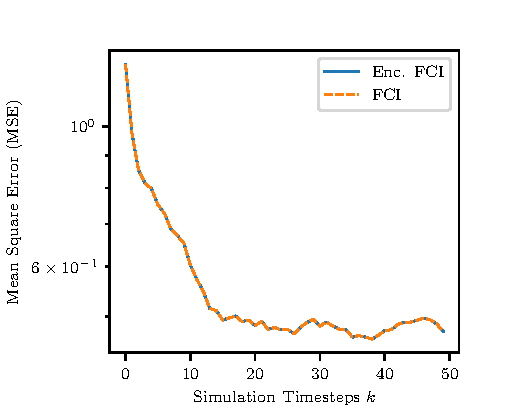
\includegraphics{figures/sim_error_plot.pdf}
    \caption{Average RMSE of encrypted and unencrypted FCI fusion over $1000$ simulations.}
    \label{fig:sim_error_plot}
\end{figure}
From the figure, we can see the expected similarity in performance between the encrypted and unencrypted FCI methods. Additionally, we note that the current recommended key length for the Paillier encryption scheme is $2048$ bits [barkerRecommendationPairWiseKey2019], easily supporting a modulus $N$ and fractional precision $\phi$ that guarantee similar performance.

% 
%  .d8888b.   .d88888b.  888b    888  .d8888b.  
% d88P  Y88b d88P" "Y88b 8888b   888 d88P  Y88b 
% 888    888 888     888 88888b  888 888    888 
% 888        888     888 888Y88b 888 888        
% 888        888     888 888 Y88b888 888        
% 888    888 888     888 888  Y88888 888    888 
% Y88b  d88P Y88b. .d88P 888   Y8888 Y88b  d88P 
%  "Y8888P"   "Y88888P"  888    Y888  "Y8888P"  
%                                               
%                                               
%                                               
% 

\section{Conclusions on Confidential Estimate Fusion}
% TODO mainly compares the two methods. One can prioritise estimates but leaks and assumes trust while the other doesn't leak but requires more computation at the query party

%FCI is a commonly used, and efficiently computable, approximation to the CI optimization problem that requires the sharing of local sensor estimates to compute their fusion. We propose a secure approximation to FCI, SecFCI, to compute the fused estimate homomorphically. The novel encrypted fusion approach may find uses in various security-critical applications or over untrusted networks subject to eavesdroppers and malicious participants. Possible future work includes run-time comparisons with FHE implementations, giving a computational bound for its practicality, and quantification of fusion weight leakages via formal security proofs.

%In this work, we have presented a method for computing encrypted Fast Covariance Intersection homomorphically on an untrusted cloud and discussed its security guarantees. The method ensures no estimator information leakage at the cloud, eavesdroppers or other estimators and an accompanying simulation demonstrates its minimal effect on estimation performance when compared to the unencrypted algorithm. Applications include a variety of distributed fusion tasks when external fusing computations are required such as weather forecasting and vehicle localisation. Future work on the topic aims to extend the method to include multivariable encryption, hiding the dimension variable $n$, and generalising to decentralised environments where individual fusing parties are untrusted.